% \documentclass[10pt]{beamer}
\documentclass[10pt,handout]{beamer}
\usepackage{BeamerColor}
\usepackage{mathtools}
\usepackage{hyperref}

\usepackage{fancybox}
\renewcommand{\indent}{\hspace*{1em}}

\mode<presentation>
{
  \usetheme{Darmstadt}      % or try Darmstadt,  Madrid,  Warsaw,  ...
 \definecolor{UBCblue}{rgb}{0.4706,  0.3725,  0.06667}
  \definecolor{ferngreen}{rgb}{0.38,  0.51,  0.71}
  \usecolortheme[named=ferngreen]{structure} % or try albatross,  beaver,  crane,  ...
  \usefonttheme{serif}  % or try serif,  structurebold,  ...
  \setbeamertemplate{navigation symbols}{}
  \setbeamertemplate{caption}[numbered]
}
%%%%%%%%%%%%%%head/foot%%%%%%%%%%%%%%%%
\setbeamertemplate{headline}{
	\begin{beamercolorbox}{section in head/foot}
%		\insertsectionnavigationhorizontal{0.94\textwidth}{}{}
\end{beamercolorbox}
}

\setbeamertemplate{footline}
    {\begin{beamercolorbox}[sep=1ex]{author in head/foot}
      %  \rlap{\tiny{}}\hfill {Y. DJEMMADA (In collaboration with A. MEHDAOUI)}\hfill\llap{\insertframenumber/\inserttotalframenumber}
       \rlap{\tiny{}}\hfill {Python programming}\hfill\llap{\insertframenumber/\inserttotalframenumber}
      \end{beamercolorbox}%
}
%%%%%%%%%%%%%%
\usepackage[english]{babel}
\usepackage[utf8]{inputenc}
\usepackage{xcolor}
\newcommand {\res}[1]{\resizebox{1\linewidth}{!}{$#1$}}
\newcommand {\tit}[1]{\begin{center}
  \shadowbox{\large \textbf{#1}}
\end{center}
}
\usepackage{tikz}
\usetikzlibrary{shapes.geometric,  arrows}
\usetikzlibrary{mindmap, trees, shadows}
\usepackage{listings}
\usepackage{yfonts} 
\usepackage[tikz]{bclogo}
\newcounter{exercise}
\setcounter{exercise}{1}
\renewcommand\bcStyleTitre[1]{\normalsize\textbf{#1 \theexercise:}\resetcounteronoverlays{exercise}
\stepcounter{exercise}}

\presetkeys{bclogo}{
epBord=1, 
couleur = red!15!white, 
couleurBord = red, 
arrondi = 0.2, 
logo=\bccrayon
}{}

\lstset
{
    language=[LaTeX]TeX, 
    breaklines=true, 
    basicstyle=\tt\scriptsize, 
    %commentstyle=\color{green}
    keywordstyle=\color{blue}, 
    %stringstyle=\color{black}
    identifierstyle=\color{magenta}, 
}
\newcommand{\ttr}[1]{  \begin{center}
  {\bf   #1    }
\end{center}
}
%\newtheorem{thm}[theorem]{Théorème}
%%%%%%%%%%%%%%%%%%%%%Theorems%%%%%%%%%%%%%%%%%%%%%%%%%%%%%%%%%%%%%%
\newenvironment<>{ex}[1]{%
  \begin{actionenv}#2%
      \def\insertblocktitle{Example}%
      \par%
      \mode<presentation>{%
       \setbeamercolor{block title}{fg=white, bg=ForestGreen!40!black}
       \setbeamercolor{block body}{fg=black, bg=green!15}
 %      \setbeamercolor{itemize item}{fg=orange!20!black}
 %      \setbeamertemplate{itemize item}[triangle]
     }%
      \usebeamertemplate{block begin}}
    {\par\usebeamertemplate{block end}
    \end{actionenv}}
\newenvironment<>{df}[1]{%
  \begin{actionenv}#2%
      \def\insertblocktitle{}%
      \par%
      \mode<presentation>{%
        \setbeamercolor{block title}{fg=black, bg=blue!15}
       \setbeamercolor{block body}{fg=black, bg=blue!15}
 %      \setbeamercolor{itemize item}{fg=orange!20!black}
 %      \setbeamertemplate{itemize item}[triangle]
     }%
      \usebeamertemplate{block begin}}
    {\par\usebeamertemplate{block end}
    \end{actionenv}}
%%%%%%%%%%%%%%%%%%%%%%%%%%%%%%%%%%%%%%%%%%%%%%%%%
\usepackage{romannum}
\usepackage[lined, boxed, commentsnumbered,  ruled, vlined, linesnumbered,  french]{algorithm2e}

%%%%%%%%%%%%%%%%%%%%
 \newtheorem{thm}{Theorem}%[section]
 \setbeamercolor{thm title}{use=structure, fg=black, bg=purple!75!black}
 \newtheorem{cor}{Corollary}%[thm]
 \newtheorem{lem}{Lemma}%[thm]
 \newtheorem{con}{Conjecture}%[thm]
 \newtheorem{prop}{Proposition}%[thm]
 \theoremstyle{definition}
 \newtheorem{dfn}{Definition}%[thm]
 \theoremstyle{remark}
 \newtheorem{rem}{Remark}%[thm]
% \newtheorem*{ex}{Example}
 \newtheorem*{pr}{\textbf{Proof}}
 \numberwithin{equation}{section}

%%%%%%%%%%%%%%%%%%
% \author{\textbf{\scriptsize Y. DJEMMADA (In collaboration with A. MEHDAOUI)}  \\ \hspace*{5cm}\\ \scriptsize{\url{yahia.djem@gmail.com} or \url{yahia.djemmada@nhsm.edu.dz}}}
\title{ \bf \huge Python Programming}
\newcommand{\D}{\mathsf{\Delta}}
\newcommand{\E}[1]{\mathsf{E}^{#1}}
\newcommand{\exercise}[1]{
\begin{bclogo}{Exercise}
#1
\end{bclogo}}
\newcommand{\dl}{\mathsf{\delta}}
% \titlegraphic {
%   \begin{minipage}{0.49\linewidth}
%   \begin{flushleft}
%   
\includegraphics[width=2cm, height=2cm, keepaspectratio]{img/3.jpg}~ 
%  \end{flushleft}
% \end{minipage}
% \begin{minipage}{0.49\linewidth}
%  \begin{flushright}
%   
\includegraphics[width=2cm, height=2cm, keepaspectratio]{img/3.jpg}~ 
%  \end{flushright}
% \end{minipage}
% }
\newcommand{\C}{\mathbb{C}}
\newcommand{\R}{\mathbb{R}}
\newcommand{\Q}{\mathbb{Q}}
\newcommand{\Z}{\mathbb{Z}}
\newcommand{\N}{\mathbb{N}}
\usepackage{datetime}
\usepackage{polynom}
\usepackage{smartdiagram}
\polyset{%
  style=D, 
  delims={\big(}{\big)}, 
  div=|
}%eucledian

\newdateformat{monthyeardate}{%
  \monthname[\THEMONTH],  \THEYEAR}

\institute{\textbf{} \\ \vspace*{0.2cm}  \scalebox{2}{\insertlogo}}
\date{}
\AtBeginSection[]
{
  \begin{frame}<beamer>
    \frametitle{Sommaire}
    \tableofcontents[currentsection, currentsubsection]
  \end{frame}
}
% Python
\usepackage{listings}
\definecolor{mygreen}{rgb}{0, 0.6, 0}
\definecolor{mygray}{rgb}{0.5, 0.5, 0.5}
\definecolor{mymauve}{rgb}{0.58, 0, 0.82}

\lstset{ %
  backgroundcolor=\color{white},    % choose the background color
  basicstyle=\footnotesize,         % size of fonts used for the code
  breaklines=true,                  % automatic line breaking only at whitespace
  captionpos=b,                     % sets the caption-position to bottom
  tabsize=1, 
  numbersep=5pt, 
  columns=fullflexible, 
  commentstyle=\color{mygreen},     % comment style
  escapeinside={\%*}{*)},           % if you want to add LaTeX within your code
  keywordstyle=\color{blue},        % keyword style
  stringstyle=\color{mymauve},      % string literal style
  framexleftmargin=5mm, 
  frame=shadowbox, 
  }

\begin{document}
\begin{frame}
\maketitle
\end{frame}
\tableofcontents
%  \include{Intro_1}
 \begin{frame}{What is Python?\footnote{https://en.wikipedia.org/wiki/Python\_(programming\_language)} }
  Python is an interpreted high-level general-purpose programming language. Its design philosophy emphasizes code readability with its use of significant indentation. Its language constructs as well as its object-oriented approach aim to help programmers write clear, logical code for small and large-scale projects.
\pause
\vspace{0.6cm}
\begin{figure}

\includegraphics[width=3.5cm,height=3.5cm,keepaspectratio]{img/python_logo.png}
\end{figure}


\end{frame}
\begin{frame}
  \tit{Who created Python?}
  Python was created by Guido van Rossum in the Netherlands in 1990. Van Rossum developed  Python as a hobby, and Python has become a popular programming language widely used in industry and academia due to its simple, concise, and intuitive syntax and extensive library.
  

\end{frame}
\begin{frame}
  \tit{Why Python?}
  Because of many reasons\footnote{https://www.quora.com/Why-do-people-still-use-Python}:
\begin{itemize}
  \item  \textbf{Easy to learn:} Learning Python is nothing but learning English.\pause
  \item  \textbf{ Used everywhere:} Python is used in AI, ML(Artificial Intelligence and Machine Learning). It is also used in data science, games, apps, websites, automation, etc.\pause
  \item  \textbf{ General purpose programming language:} It is a general purpose programming language which means it can be used on all devices and also in many different situations.\pause
  \item  \textbf{ Loads of libraries:} Want to solve algebraic equations? Use numpy. Want to deal with images? Use PIL.\pause
  \item \textbf{Just few lines of code does great:} With Python in just 5 lines of code is equivalent to, say, 20 lines of PHP code.\pause
  \item  \textbf{ Great community:} Many people are willing to help with issues regarding Python. There is a great community.
    
\end{itemize}

\end{frame}
\begin{frame}
  \tit{Why Python?\footnote{https://becominghuman.ai/why-is-python-so-popular-b01a006b2be4}}

 \begin{center}
    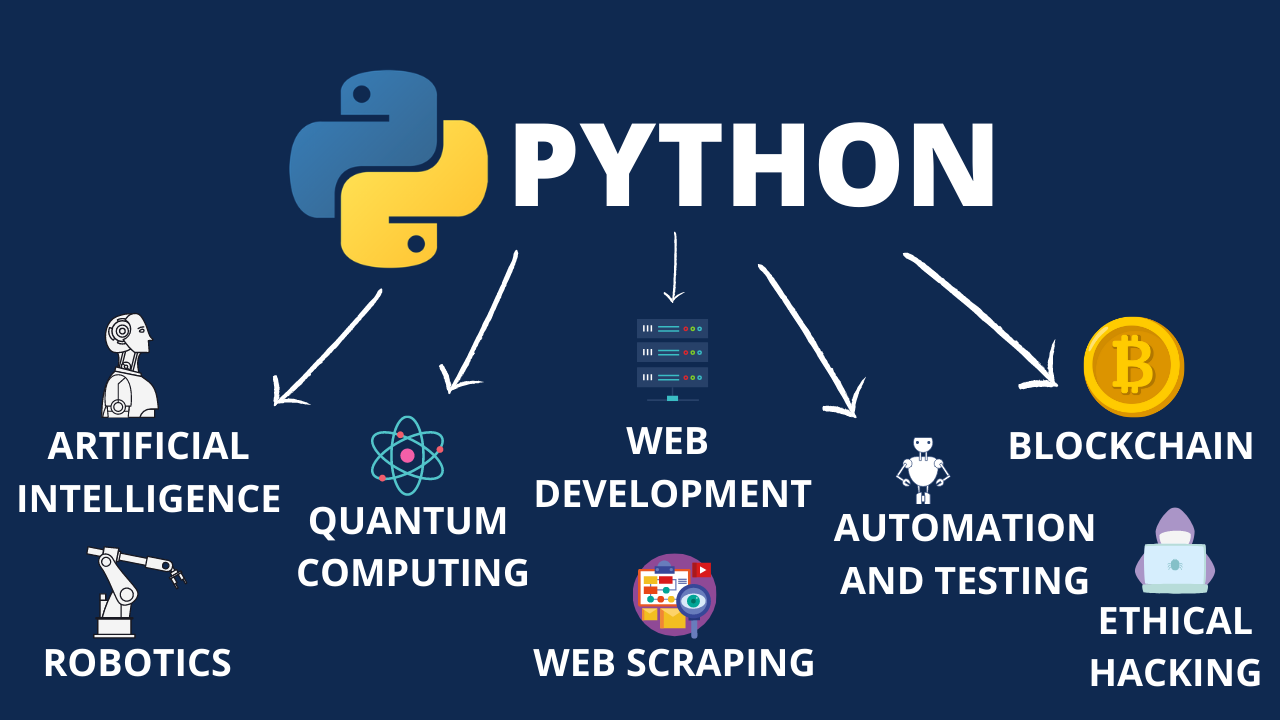
\includegraphics[scale=0.25]{img/why_python.png}
 \end{center}

\end{frame}
\begin{frame}
  \tit{Why Python?}

 \begin{center}
    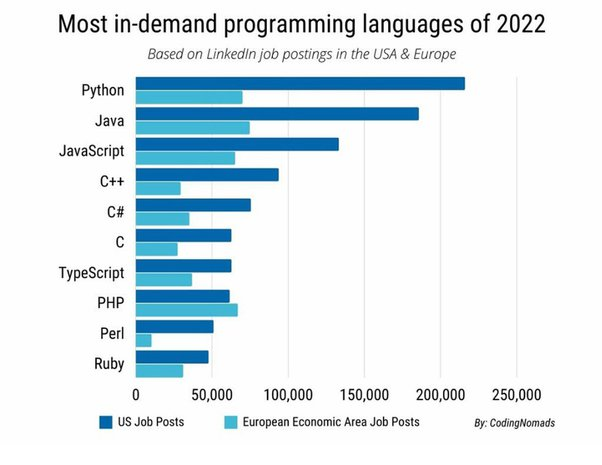
\includegraphics[scale=0.5]{img/most_demand.jpeg}
 \end{center}

\end{frame}
\begin{frame}
  \tit{Why Python?}

 \begin{center}
    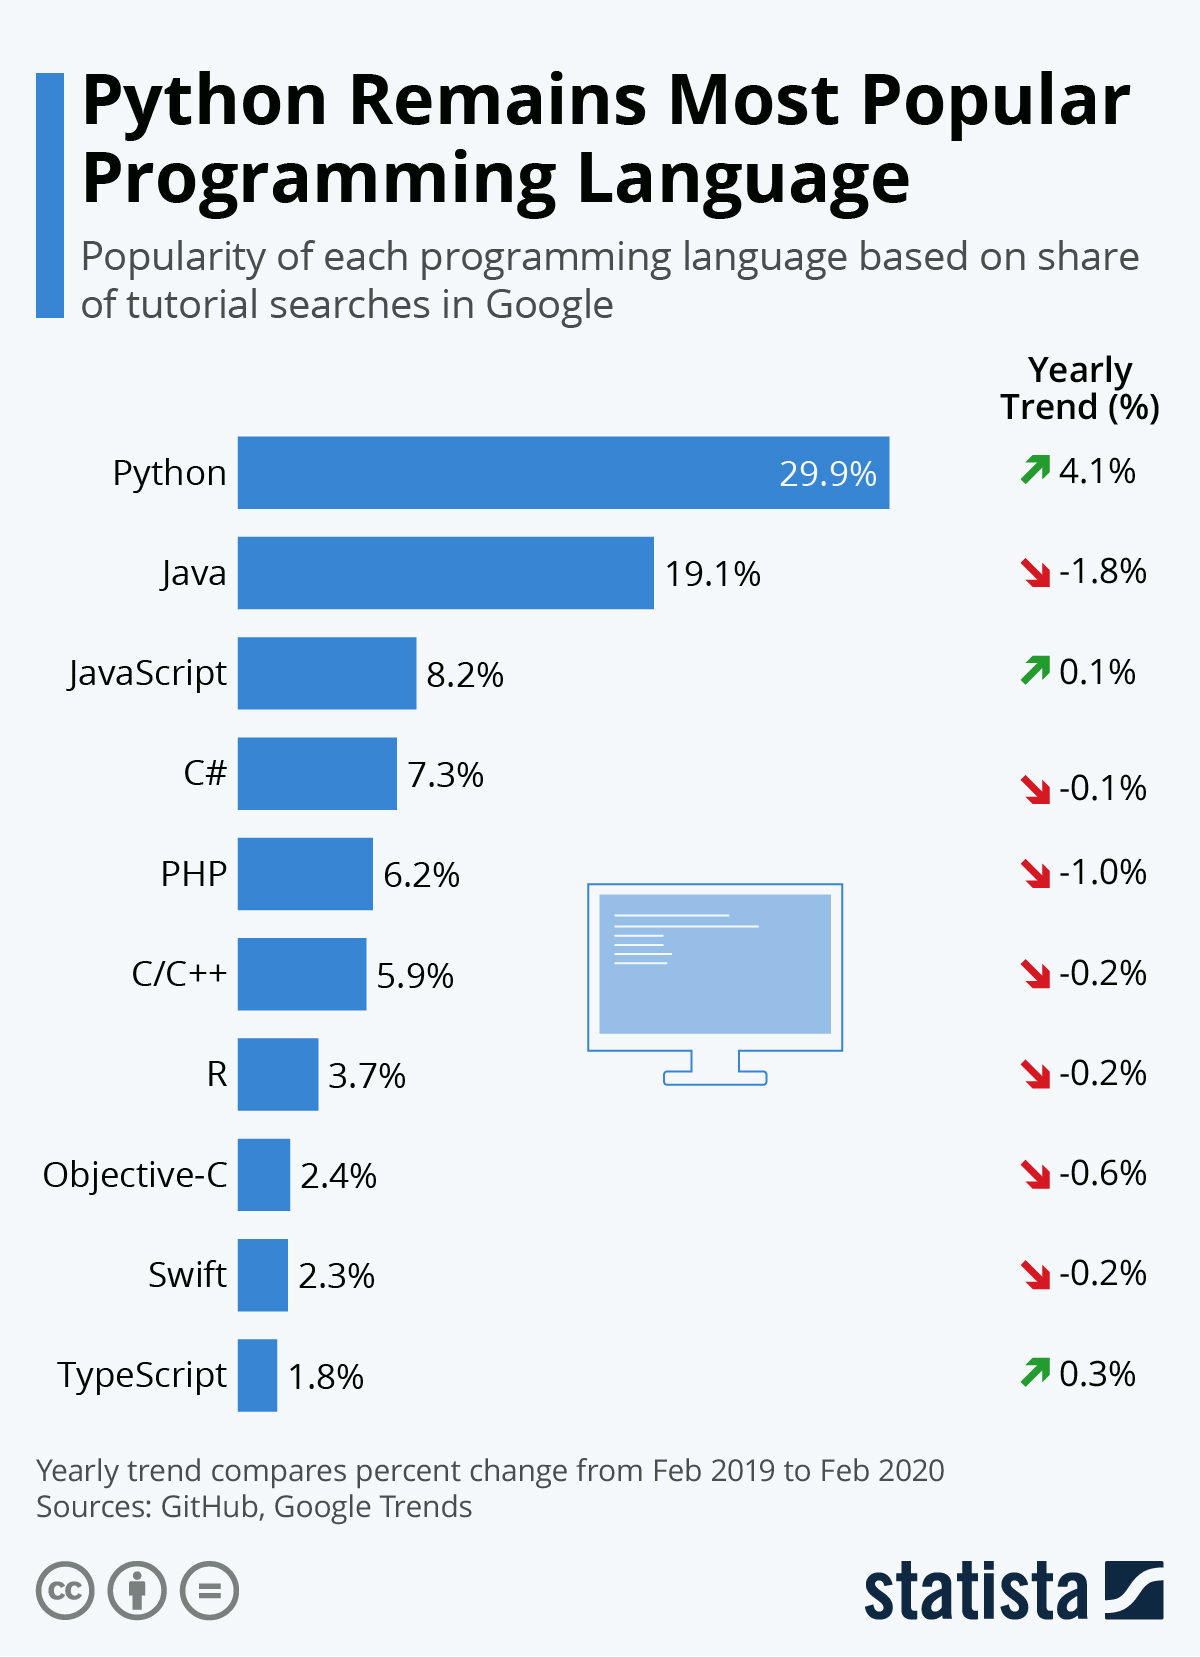
\includegraphics[scale=0.13]{img/most_popular.jpeg}
 \end{center}

\end{frame}
\begin{frame}
  \tit{What is an open source/free software?\footnote{https://en.wikipedia.org/wiki/Free\_and\_open-source\_software}}
  Free and open-source software (FOSS) is software that is both free software and open-source software[a] where anyone is freely licensed to use, copy, study, and change the software in any way, and the source code is openly shared so that people are encouraged to voluntarily improve the design of the software.
  \pause \\
  Examples of free software: \textbf{VLC Media}, \textbf{Linux Mint}, \textbf{Gimp}, \textbf{Firefox}, ... etc.

% \end{frame}
% \begin{frame}{Logiciel Libre \footnote{https://en.wikipedia.org/wiki/Free\_software}}
%   Free software (or libre software) is computer software distributed under terms that allow users to run the software for any purpose as well as to study, change, and distribute it and any adapted versions. 
% \pause
\vspace{1cm}
\begin{figure}

\includegraphics[width=3cm,height=2.5cm,keepaspectratio]{img/gnu.png}
\end{figure}

\end{frame}
\begin{frame}{What is a Licence?}
  A software license is a contract by which the copyright holder of a computer program defines with his co-contractor (operator or user) the conditions under which this program may be used, distributed or modified.
\end{frame}
\begin{frame}{GNU Licence\footnote{https://en.wikipedia.org/wiki/GNU\_General\_Public\_License}}
  The GNU General Public License (GNU GPL or simply GPL) is a series of widely used free software licenses that guarantee end users the four freedoms to run, study, share, and modify the software.

\pause
\vspace{1cm}
\begin{figure}

\includegraphics[width=3cm,height=2.5cm,keepaspectratio]{img/GPLv3.png}
\end{figure}

\end{frame}
\begin{frame}
  \tit{Levels of freedom of a software}
\pause
  \begin{center}
      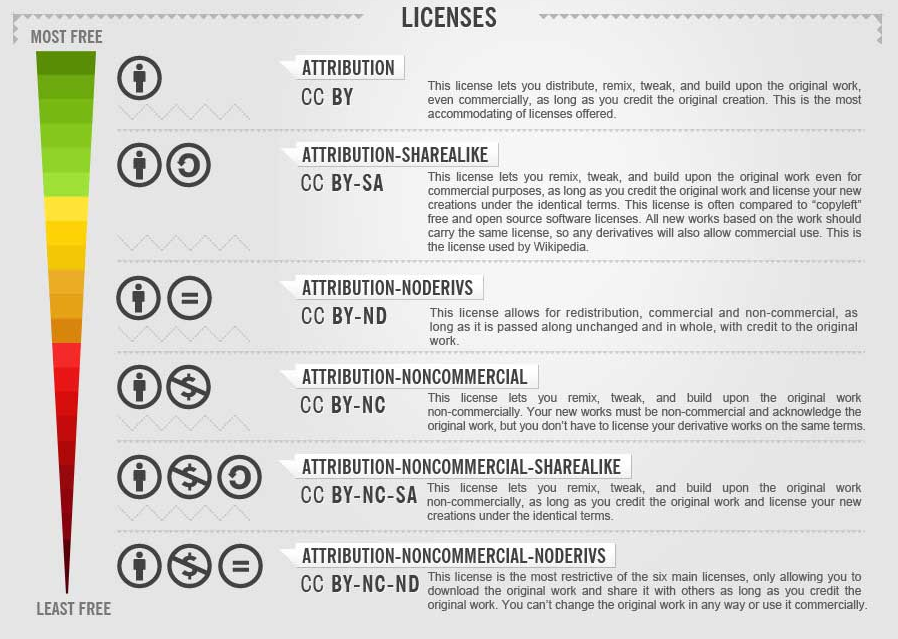
\includegraphics[scale=0.44]{img/creative-commons2.png}
  \end{center}


\end{frame}
\begin{frame}
  \tit{Is there other types of licences?}
\pause
\begin{center}
      \includegraphics[scale=0.3]{img/table_comp.png}
\end{center}
\end{frame}
\begin{frame}
  \tit{What we will study during the semester}

\begin{center}
  \resizebox{.5\linewidth}{!}{
  \smartdiagram[descriptive diagram]{
    {Chap 1,{Introduction to computers, Programs and Python}},
    {Chap 2, {Elementary Programming}}, 
    {Chap 3, {Mathematical Functions and Strings}},
    {Chap 4,{ Conditions}},
    {Chap 5, {Loops}}, }}
\end{center}

\end{frame}
\begin{frame}
  \tit{What we will study during the semester}
\begin{center}
  \resizebox{.5\linewidth}{!}{
  \smartdiagram[descriptive diagram]{
    {Chap 6, Functions},
    {Chap 7, Lists},
    {Chap 8, {Tuples, Sets and Dictionaries}},
    {Chap 9, Multidimensional Lists},
    {Chap 10, Files and Exceptions Handling}}}
\end{center}

\end{frame}
% \begin{frame}
%   \tit{Python 2 Vs Python 3}

  

% \end{frame}
\begin{frame}
  \tit{Differents ways to run Python}

\begin{itemize}
  \item Interactive Mode (Command prompt).\pause
  \item Command Line (File running)  'python file.py'. \pause
  \item Text Editor (VS Code, Jupyter). \pause
  \item IDE (PyCharm)
\end{itemize}
  

\end{frame}
\begin{frame}
  \tit{Type of Errors}

  \begin{itemize}
    \item \textbf{Syntax errors} result from errors in code construction, such as mistyping a statement, incor-
rect indentation, omitting some necessary punctuation, or using an opening parenthesis with-
out a corresponding closing parenthesis.
    \item \textbf{Runtime errors} are errors that cause a program to terminate abnormally. They occur while a
    program is running if the Python interpreter detects an operation that is impossible to carry
    out.
    \item \textbf{Logic errors} occur when a program does not perform the way it was intended to. Errors of this
    kind occur for many different reasons.
  \end{itemize}

\end{frame}
\begin{frame}
  \tit{Objective of the course}
\begin{block}
  
    At the end of this semester, you will be able to solve a problem and write its code in Python.
  
\end{block}
\end{frame}
 \begin{frame}[fragile]{Elementary programming}
    \tit{Comments}
    All modern programming languages have comment characters. These indicate part of
    the code that should be skipped by the interpreter.
    \tit{Why comments !}
    \begin{itemize}[<+->]
        \item Comments can be used to explain Python code.

        \item Comments can be used to make the code more readable.
        
        \item Comments can be used to prevent execution when testing code.
    \end{itemize}
    \pause
    \tit{How we write comments ?}
    \begin{block}{}
        Any characters after a sharp ({\bf \#}) on a line are skipped.
    \end{block}

\end{frame}
\begin{frame}[fragile]{Elementary programming}
\begin{lstlisting}[numbers=left,showstringspaces=false,language=python]
#This is a comment
#written in
#more than just one line
print("Hello, NHSM!")
#print("This line will be ignored ")
print("Did you understand comments ?") #This line will print "Did ...?" 
\end{lstlisting}
\pause
\tit{Python multiline comments}
Python doesn't support multiline comments.

However, you can use two triple quotes (""") as multiline comments.

Guido van Rossum, the creator of Python, also recommended this.
\pause
\begin{lstlisting}[numbers=left,showstringspaces=false,language=python]
    """ This is a comment
    written in
    more than just one line
    """
    print("Hello, NHSM!")
\end{lstlisting}
\end{frame}
\begin{frame}[fragile]{Elementary programming}
    \tit{Variables assignement}
\begin{block}{}
    Variables consist of two parts: the identifier (name)  and the value.
\end{block}


To assign a variable to a name, use a single equals sign ( = ).


A variable is created the moment you first assign a value to it.
\pause 
\begin{lstlisting}[numbers=left,showstringspaces=false,language=python]
Name = "Omar" #Create a variable named 'Name' with String value 'Omar'
Age = 5 #Create a variable named 'Age' with Integer value '25'
High = 1.73 #Create a variable named 'Age' with real value '1.73'
\end{lstlisting}
\pause 
Python allows you to assign a single or multiple values (not mandatory of the same type) to several variables simultaneously.
\begin{lstlisting}[numbers=left,showstringspaces=false,language=python]
a = b = c = 10 #assign a single 10 to a,b and c
Name,Age,High = "Omar",2,1.73 #assign 3 different values to 3 variables.
\end{lstlisting}
\end{frame}

\begin{frame}[fragile]{Elementary programming}
\tit{Type of variable}
You don’t do this in Python, however, because Python automatically figures out
the data type according to the value assigned to the variable.

\pause 
The most used types in Python are: 
\begin{lstlisting}[numbers=left,showstringspaces=false,language=python]
int #numerical type
float #numerical type
str #for textual manipulation
bool #logical type
complex #numerical type
\end{lstlisting}
You can determine the type of a variable or a literal
value by using the \lstinline{type()} function.
\begin{lstlisting}[numbers=left,showstringspaces=false,language=python]
>>> High = 1.73 
>>> type(High)
<class 'float'>
>>> type(43)
<class 'int'>
\end{lstlisting}
\end{frame}
\begin{frame}[fragile]{Elementary programming}
\tit{type conversion}
You can convert from one type to another with the \verb|int()|, \verb|float()|, and \verb|complex()| methods:
\begin{lstlisting}[numbers=left,showstringspaces=false,language=python]
x = 5    # int
y = 1.81  # float
z = 3+1j   # complex

#convert from int to float:
a = float(x)
#convert from float to int:
b = int(y)
#convert from int to complex:
c = complex(x)

print(a)
print(b)
print(c)

print(type(a))
print(type(b))
print(type(c))
\end{lstlisting}

\end{frame}
\begin{frame}[fragile]{Elementary programming}
    \tit{Dynamic types of variables}
Python is dynamically typed. This means that:
\begin{itemize}[<+->]
    \item Types are set on the variable values and not on the variable names.
    \item Variable types do not need to be known before the variables are used.
    \item Variable names can change types when their values are changed.
\end{itemize}
\onslide<4->
\begin{lstlisting}[numbers=left,showstringspaces=false,language=python]
a=3
a="yes"
a=1.73
\end{lstlisting}
\end{frame}
\begin{frame}[fragile]{Elementary programming}
\tit{Naming variables}
    \begin{itemize}[<+->]
        \item Variable names can contain only letters, numbers, and underscores \verb|(_)|.
         They can start with a letter or an underscore \verb|(_)|, not with a number.
        \item Variable names cannot contain spaces. To separate words in variables, you use underscores for example \verb|sorted_list|
        \item Variable names cannot the same as keywords, reserved words, and built-in functions in Python.
        \end{itemize}
        \onslide<4->{The following guidelines help you define good variable names:}
        \begin{itemize}[<+->]
            \item Variable names should be concise and descriptive. For example, the \verb|active_user| variable is more descriptive than the \verb|au|.
            \item Use underscores \verb|(_)| to separate multiple words in the variable names.
            \item Avoid using the letter \verb|l| and the uppercase letter \verb|O| because they look like the number \verb|1| and \verb|0|.
        \end{itemize}
\end{frame}
\begin{frame}[fragile]{Elementary programming}
    \tit{Operators \& Evaluating expressions}
    \begin{block}{}
        Operators are the syntax that Python uses to express common ways to manipulate
data and variables.
    \end{block}
    Python divides the operators in the following groups:
    \begin{center}{\bf Arithmetic operators}\end{center}
    Arithmetic operators are used with numeric values to perform common mathematical operations:
    \begin{center}
        \begin{tabular}{ |  p{3cm} | p{3cm} | p{3cm} |}
            \hline
            Operator &Name&Usage\\
            \hline
        \verb|+| & Addition & \verb|x + y|\\  
        \verb|-| & Subtraction & \verb|x - y|\\  
        \verb|*| & Multiplication & \verb|x * y|\\  
        \verb|/| & Float Division & \verb|x / y|\\  
        \verb|%| & Remainder & \verb|x % y|\\  
        \verb|**| & Exponentiation & \verb|x ** y|\\  
        \verb|//| & Integer division & \verb|x // y|\\
        \hline
        \end{tabular}
    \end{center}
\end{frame}
\begin{frame}[fragile]{Elementary programming}
    \tit{Operators \& Evaluating expressions}
    \begin{center}{\bf Assignment operators}\end{center}
    Assignment operators are used to assign values to variables:
    \begin{center}
        \begin{tabular}{ |  p{3cm} | p{4cm} | p{3cm} |}
            \hline
            Operator &Name&Usage\\
            \hline
            \verb|=|&\text{assignment}&\verb|x=3|\\
            \verb|+=|&\text{addition assignment}&\verb|x+=3|\\
            \verb|-=|&\text{subtraction assignment}&\verb|x-=3|\\
            \verb|*=|&\text{multiplication assignment}&\verb|x*=3|\\
            \verb|/=|&\text{float division assignment}&\verb|x/=3|\\
            \verb|//=|&\text{integer division assignment}&\verb|x//=3|\\
            \verb|%=|&\text{remainder assignment}&\verb|x%=3|\\
            \verb|**=|&\text{exponent assignment}&\verb|x**=3|\\
            \hline
        \end{tabular}
    \end{center}
\end{frame}
\begin{frame}[fragile]{Elementary programming}
    \tit{Operators \& Evaluating expressions}
    \begin{center}{\bf Relational operators}\end{center}
    Logical operators are used to combine conditional statements:

    \begin{center}
        \begin{tabular}{ |  p{3cm} | p{4cm} | p{3cm} |}
            \hline
            Operator &Name&Usage\\
            \hline
            \verb|<|&\text{less than}&\verb|x<y|\\
            \verb|<=|&\text{less than or equal to}&\verb|x<=y|\\
            \verb|>|&\text{greater than}&\verb|x>y|\\
            \verb|>=|&\text{greater than or equal to}&\verb|x>=y|\\
            \verb|==|&\text{equal to}&\verb|x==y|\\
            \verb|!=|&\text{not equal}&\verb|x!=y|\\
            \hline
        \end{tabular}
    \end{center}
\end{frame}

\begin{frame}[fragile]{Elementary programming}
    \tit{Operators \& Evaluating expressions}
    \begin{center}{\bf Logical operators}\end{center}

    Logical operators are used to combine conditional statements:

    \begin{center}
    \begin{tabular}{ |  p{2cm} | p{3cm} | p{4cm} |}
        \hline
        Operator &Name&Usage\\
        \hline
        \verb|and|&\text{logical conjunction}&\verb|x < 5 and  x < 10|\\
        \verb|or|&\text{logical disjunction}&\verb|x < 5 or x < 4|\\ 
        \verb|not|&\text{logical negation}&\verb|not(x < 5 and x < 10)|\\
        \hline
    \end{tabular}
\end{center}
\end{frame}
\begin{frame}[fragile]{Elementary programming}
\tit{Python Operators Precedence Rule}
\begin{itemize}[<+->]
    \item An expression is made with combinations of variables, values, operators and function calls.
    
    
    \item The Python interpreter evaluates the valid expression.
    
    
    \item Python uses a type of rule known as {\bf PEMDAS}.
\begin{enumerate}[<+->]
     \item {\bf P}:  Parentheses
    \item {\bf E}:  Exponentiation
    \item {\bf M}:  Multiplication
    \item {\bf D}:  Division
    \item {\bf A}:  Addition
    \item {\bf S}:  Subtraction
\end{enumerate}
\item Operators with the same precedence (except for \verb|**|) are evaluated from left-to-right.
\end{itemize}
\end{frame}
\begin{frame}[fragile]{Elementary programming}
    \tit{Input / output data}
    \begin{lstlisting}[numbers=left,showstringspaces=false,language=python]
        Age=eval(input("How old are you ?"))# input statement
        print(Age)#Output (display) statement
    \end{lstlisting}
\end{frame}
\begin{frame}[fragile]{Elementary programming}
    \tit{Types of Errors}
    \begin{center}{\bf Syntax Errors}\end{center}
  Syntax errors are the most basic type of error. They arise when the Python parser is unable to understand a line of code. Syntax errors are almost always fatal, i.e. there is almost never a way to successfully execute a piece of code containing syntax errors
\end{frame}
\begin{frame}[fragile]{Elementary programming}
  
\begin{center}{\bf Runtime Errors}\end{center}

 A program with a runtime error is one that passed the interpreter's syntax checks, and started to execute. However, during the execution of one of the statements in the program, an error occurred that caused the interpreter to stop executing the program and display an error message.  Runtime errors are also called exceptions because they usually indicate that something exceptional (and bad) has happened.



 Some examples of Python runtime errors:
 \begin{enumerate}[<+->]
   \item  division by zero 
   \item performing an operation on incompatible types 
   \item using an identifier which has not been defined 
   \item accessing a list element, dictionary value or object attribute which doesn't exist 
   \item trying to access a file which doesn't exist    
 \end{enumerate}

\end{frame}
\begin{frame}[fragile]{Elementary programming}
\begin{center}{\bf Logic Errors}\end{center}
These are the most difficult type of error to find, because they will give unpredictable results and may crash your program.  A lot of different things can happen if you have a logic error. However these are very easy to fix as you can use a debugger, which will run through the program and fix any problems.


Here are some examples of mistakes which lead to logical errors: 
\begin{enumerate}[<+->]
  \item using the wrong variable name
  \item indenting a block to the wrong level
  \item using integer division instead of floating point division
  \item getting operator precedence wrong
  \item  making a mistake in a boolean expression
  \item off-by-one, and other numerical errors
\end{enumerate}
\end{frame}
\begin{frame}[fragile]{Elementary programming}
    \tit{Documentation}
   There is online and offline versions of Python documentation 
   \begin{itemize}
     \item online: \url{https://www.python.org/doc/}
     \item offline: Zeal \url{https://zealdocs.org/}
   \end{itemize}
  \end{frame}
  \begin{frame}[fragile]{Elementary programming}
    \tit{How to find a solution for a problem}
  \begin{itemize}
    \item Write the Errors on Google as it is.
    \item Ask a question on a forum.
  \end{itemize}
  \end{frame}
% \begin{frame}[fragile]{Elementary programming}
% \end{frame}
% \begin{frame}[fragile]{Elementary programming}
% \end{frame}
% \begin{frame}[fragile]{Elementary programming}
% \end{frame}
% \begin{frame}[fragile]{Elementary programming}
% \end{frame}
% \begin{frame}[fragile]{Elementary programming}
% \end{frame}


%Elementary programming 
%TODO: Talk about errors
 \begin{frame}[fragile]{Math functions and Strings}
\tit{Mathematical functions}
Python has a limited number of {\bf built-in mathematical functions}:
    \begin{lstlisting}[numbers=left,showstringspaces=false,language=python]
    abs( number ) #Return the absolute value of the argument, |x|.
    pow( x , y , [ z ]) #Raise x to the y power. If z is present, this is done 
                      #modulo z , x y % z .
    round( number , [ ndigits ]) #Round number to ndigits beyond the decimal 
                                #point (rounds a number to the nearest 
                                #whole number).
    cmp( x , y ) #Compare x and y , returning a number.     
    hex( number )#Create a hexadecimal string representation of number . A 
                   #leading '0x' is placed on the string as a reminder that 
                   #this is hexadecimal.
    oct( number )#Create a octal string representation of number .
                  #A leading '0' is placed on the string as a reminder that this
                  #is octal not decimal. 
    int( string , [ base ]) #Generates an integer from the string x . If base is
                         #supplied, x must be in the given base. If base is 
                         #omitted, x must be decimal.
    max( sequence ) #Return the largest value in sequence .
    min( sequence ) #Return the smallest value in sequence .
    ord( character ) #Returns the Unicode code from a given character. 
    chr( character ) #Returns a character whose Unicode code point is an integer.
    \end{lstlisting}      
\end{frame}
\begin{frame}[fragile]{Math functions and Strings}
    \tit{ math module functions}
More advanced mathematical functions are contained in the {\bf \verb|math| module}.


A {\bf module} is a file that contains a collection of related functions.

Before we can use the functions from a module, we have to import them:
\begin{lstlisting}[numbers=left,showstringspaces=false,language=python]
import math # call module before use
angle = 90 * 2 * math.pi / 360.0
math.sin(angle)
\end{lstlisting}
\end{frame}
\begin{frame}[fragile]{Math functions and Strings}
    \tit{Examples}
\begin{lstlisting}[numbers=left,showstringspaces=false,language=python]
math.ceil(x) #Returns the smallest integer greater than or equal to x.
math.fabs(x) #Returns the absolute value of x
math.factorial(x) #Returns the factorial of x
math.floor(x) #Returns the largest integer less than or equal to x
math.fmod(x, y) #Returns the remainder when x is divided by y
math.exp(x) #Returns e**x
math.log(x[, b]) #Returns the logarithm of x to the base b (defaults to e)
math.log2(x) #Returns the base-2 logarithm of x
math.log10(x) #Returns the base-10 logarithm of x
math.pow(x, y) #Returns x raised to the power y
math.sqrt(x) #Returns the square root of x
math.acos(x) #Returns the arc cosine of x
math.asin(x) #Returns the arc sine of x
math.atan(x) #Returns the arc tangent of x
\end{lstlisting}
\end{frame}
\begin{frame}[fragile]{Math functions and Strings}
    \tit{Examples}
    \begin{lstlisting}[numbers=left,showstringspaces=false,language=python]
math.cos(x) #Returns the cosine of x
math.sin(x) #Returns the sine of x
math.tan(x) #Returns the tangent of x
math.degrees(x)	#Converts angle x from radians to degrees
math.radians(x)	#Converts angle x from degrees to radians
math.acosh(x) #Returns the inverse hyperbolic cosine of x
math.asinh(x) #Returns the inverse hyperbolic sine of x
math.atanh(x) #Returns the inverse hyperbolic tangent of x
math.cosh(x) #Returns the hyperbolic cosine of x
math.sinh(x) #Returns the hyperbolic cosine of x
math.tanh(x) #Returns the hyperbolic tangent of x
math.pi	#Mathematical constant, the ratio of circumference of a 
        #circle to it's diameter (3.14159...)
math.e #Mathematical constant e (2.71828...)
\end{lstlisting}
\end{frame}
\begin{frame}[fragile]{Math functions and Strings}
    \tit{What is String in Python?}
    A string is a sequence of characters.

    \tit{How to create a string in Python?}
    Strings can be created by enclosing characters inside a single quote or double-quotes.
    
    
    Even triple quotes can be used in Python but generally used to represent multiline strings and docstrings.
\begin{lstlisting}[numbers=left,showstringspaces=false,language=python]
    # defining strings in Python, all of the following are equivalent
    say_hello = 'Hello'

    say_hello = "Hello"

    say_hello = '''Hello'''
    
    # triple quotes string can extend multiple lines
    say_hello = """Hello, welcome to
               the world of Python"""
\end{lstlisting}
\end{frame}
\begin{frame}[fragile]{Math functions and Strings}
\tit{How to access characters in a string?}
\begin{itemize}[<+->]
    \item We can access individual characters using {\bf indexing} and a range of characters using {\bf slicing}. 
    
    
    \item Python is zero-indexing language, Index starts from 0. 
    
    \item Trying to access a character out of index range will raise an \verb|IndexError|.
    \item The index must be an integer. We can't use floats or other types, this will result into \verb|TypeError|.
   \item Python allows negative indexing for its sequences.
   \item The index of $-1$ refers to the last item, $-2$ to the second last item and so on. We can access a range of items in a string by using the slicing operator :(colon).
\end{itemize}
\end{frame}
\begin{frame}[fragile]{Math functions and Strings}
\begin{lstlisting}[numbers=left,showstringspaces=false,language=python]
#Accessing string characters in Python
my_word = 'ThisIsALongWord'
print('my_word = ', my_word)

#first character
print('my_word[0] = ', my_word[0])

#last character
print('my_word[-1] = ', my_word[-1])

#slicing 2nd to 5th character
print('my_word[1:5] = ', my_word[1:5])

#slicing 6th to 2nd last character
print('my_word[5:-2] = ', my_word[5:-2])
\end{lstlisting}
\pause
Now, we try to access an index out of the range or use numbers other than an integer
\begin{lstlisting}[numbers=left,showstringspaces=false,language=python]
# index must be in range
my_word[16]  
# index must be an integer
my_word[1+0j] 
\end{lstlisting}

\end{frame}
\begin{frame}[fragile]{Math functions and Strings}
    \tit{Common Operations on Strings}
    {\center \bf Concatenation of Two or More Strings\\}
        Joining of two or more strings into a single one is called concatenation.


        The \verb|+| operator does this in Python. Simply writing two string literals together also concatenates them.

        The \verb|*| operator can be used to repeat a string for a given number of times.
\begin{lstlisting}[numbers=left,showstringspaces=false,language=python]
# Python String Operations
str1 = 'Hello'
str2 ='NHSM!'

# using +
print('str1 + str2 = ', str1 + str2)
# using *
print('str2 * 3 =', str2 * 3)
# two string literals together
str1='Hello ''World!'
print('str1  =', str1)
\end{lstlisting}
\end{frame}
\begin{frame}[fragile]{Math functions and Strings}

    {\center \bf String Membership Test\\}

    We can test if a substring exists within a string or not, using the keyword \verb|in|
\begin{lstlisting}[numbers=left,showstringspaces=false,language=python]
    'me' in 'home'
    'ho' not in 'home'
\end{lstlisting}
{\center \bf Built-in functions to Work with Python\\}
The \verb|enumerate()| function returns an enumerate object.


The \verb|len()| returns the length (number of characters) of the string.
\begin{lstlisting}[numbers=left,showstringspaces=false,language=python]
    word="Hello NHSM"
    print(enumerate(word))
    print(len(word))
\end{lstlisting}
\end{frame}
\begin{frame}[fragile]{Math functions and Strings}
    {\center \bf Common String methods\\}
    Some of the commonly used methods are \verb|lower()|, \verb|upper()|, \verb|join()|, \verb|split()|, \verb|find()|, \verb|replace()| etc. 
    \begin{lstlisting}[numbers=left,showstringspaces=false,language=python]
        word="PythonIsNotFunny"
        print(word.lower())
        print(word.upper())
        sentence="This will split all words into a list"
        print(sentence.split())
        sentence="This will split, all words, into a list"
        print(sentence.split(','))
        word_list=['This', 'will', 'join', 'all', 'words', 'into', 'a', 'string']
        delimiter="*"
        print(delimiter.join(word_list))
        print(' '.join(word_list))
        print('Happy Day with python'.find('ay'))
        print('Happy Day with python'.replace('Happy','Brilliant'))
    \end{lstlisting}
\end{frame}
%Math functions & Strings
%TODO: Common errors in Strings 
%TODO: print("", end=)
%TODO: string format
%TODO: raw_input("Give").split()
\begin{frame}[fragile]{Indentation}
    \tit{Python Indentation}
    Indentation is a very important concept of Python because without proper indenting the Python code, 
    you will end up seeing IndentationError and the code will not get compiled.



    In simple terms indentation refers to adding white space before a statement.
    \pause
    \begin{lstlisting}[numbers=left,showstringspaces=false,language=python]
        Username = 'Omar_213'  
        if Username == 'Omar_213': 
            print('Logging on to website...')
            password=input('Enter your password') 
        else: 
            print('You are in the wrong place.') 
        print('All set !')
        \end{lstlisting}        
\end{frame}
\begin{frame}[fragile]{Indentation}
    \tit{Python Indentation Rules}
Python uses 4 spaces as default indentation spaces. However, the number of spaces can be anything, it is up to the user. 
But a minimum of one space is needed to indent a statement.
\begin{itemize}
    \item The first line of python code cannot have Indentation.
    \item Indentation is mandatory in python to define the blocks of statements.
    \item The number of spaces must be uniform in a block of code.
    \item It is preferred to use whitespaces instead of tabs to indent in python. Also, either use whitespace or tabs to indent, intermixing of tabs and whitespaces in indentation can cause wrong indentation errors.
\end{itemize}
\end{frame}
\begin{frame}[fragile]{Indentation}
\tit{Benefits of Indentation in Python}
\begin{itemize}
    \item Indentation of code leads to better readability, although the primary reason for indentation in python is to identify block structures.
    \item Missing \verb|{| and \verb|}| errors that sometimes popup in \verb|c,c++| languages (or other languages) can be avoided in python, also the number of lines of code is reduced.
\end{itemize}
\end{frame}
%TODO: if...else 
    %*Syntax
    %*Example
    %*Common Errors
\begin{frame}[fragile]{Conditions}
    \tit{\texttt{if} statement}
    Some programming problems need special treatment. 
    
    
    Let consider the following situation:
\begin{block}{}
Write a program that asks the user's age, then prints out the message "You are still young!" if his age is less than 30.
\end{block}
\pause 
to solve this problem, we need to use \texttt{if} statement given by the following syntax:
\begin{lstlisting}[numbers=left,showstringspaces=false,language=python] 
    if (test): #condition
        block of instructions #body
\end{lstlisting}
    \pause
\begin{itemize}[<+->]
    \item An \verb|if| statement executes the statements if the condition is true, and ignores it if the condition is false.
    \item The block of instructions must starts with and indentation and will end at the first unindented statement. 
\end{itemize}
\end{frame}
\begin{frame}[fragile]{Conditions}
    \begin{figure}
        \begin{center}
            \resizebox{.3\linewidth}{!}{
    
    \tikzstyle{decision} = [diamond, aspect=2, align=center, draw, fill=green!20, 
        text width=5.5em, text badly centered, node distance=2.5cm, inner sep=0pt]
    \tikzstyle{block} = [rectangle, aspect=2, align=center, draw, fill=blue!20, 
        text width=5em, text centered, rounded corners, minimum height=3em]
    \tikzstyle{line} = [draw, -latex']
    \tikzstyle{cloud} = [draw, ellipse,fill=red!20]
        
    \begin{tikzpicture}[node distance = 1.5cm, auto]
        % Place nodes
        \node [cloud] (init) {begin if};
        \node [decision,below of=init] (test) {test (condition)};
        \node [block, below of=test, node distance=2.5cm] (body) {body};
        \node [cloud, below of=body] (end) {end if};
        % Draw edges
        \path [line,dashed] (init) -- (test);
        \draw [line]  (test) --node[right] {True}  (body);
        \draw [line]  (test.west) |- (-2,-2.5) node[left] {False} |- (end.west);
        \path [line] (body) -- (end);
    \end{tikzpicture}}
    \end{center}
    \caption{Python \texttt{if} Statement Flowchart}
    \end{figure}
    \pause

    Therefore, the solution of the previous situation is:
\begin{lstlisting}[numbers=left,showstringspaces=false,language=python]
age=int(input("How old are you")) 
if (age<30):
    print("You are still young!")
\end{lstlisting}

\end{frame}
\begin{frame}[fragile]{Conditions}
\tit{\texttt{if...else} statements}
\begin{minipage}{.49\textwidth}
 \begin{block}{}
        If we have two outputs based on whether
        the condition is true or false,  we use the \fbox{\texttt{if...else}} statements
        \pause 
        \begin{itemize}[<+->]
            \item When the condition evaluates to \texttt{True}  executes the \fbox{\texttt{body\_of\_if}} and the \fbox{\texttt{body\_of\_else}} is skipped.
            \item When the condition evaluates to \texttt{False}
        the \fbox{\texttt{body\_of\_if}} is skipped and the \fbox{\texttt{body\_of\_else}} executes.
        \end{itemize}
 \end{block}
\end{minipage}
\begin{minipage}{.5 \textwidth}
    \begin{figure}
        \begin{center}
            \resizebox{.6\linewidth}{!}{
    \tikzstyle{decision} = [diamond, aspect=2, align=center, draw, fill=green!20, 
        text width=5.5em, text badly centered, node distance=2.5cm, inner sep=0pt]
    \tikzstyle{block} = [rectangle, aspect=2, align=center, draw, fill=blue!20, 
        text width=5em, text centered, rounded corners, minimum height=3em]
    \tikzstyle{line} = [draw, -latex']
    \tikzstyle{cloud} = [draw, ellipse,fill=red!20]    
    \begin{tikzpicture}[node distance = 1.5cm, auto]
        % Place nodes
        \node [cloud] (init) {begin if};
        \node [decision,below of=init] (test) {test (condition)};
        \node [block, below of=test, node distance=2.5cm] (body1) {body if};
        \node [block, below of=body1, node distance=2.5cm] (body2) {body else};
        \node [cloud, below of=body2] (end) {end if};
        % Draw edges
        \path [line,dashed] (init) -- (test);
        \draw [line]  (test) -- (body1);
        \draw [line]  (test.west) |- (-2,-2.5) node[left] {False} |- (body2.west);
        \path [line] (body1.east) |-(2,-5)|- (end.east);
        \path [line] (body2) -- (end);
    \end{tikzpicture}}
    \end{center}
    \caption{\texttt{if..else} Flowchart}
    \end{figure}
\end{minipage}
\end{frame}
\begin{frame}[fragile]{Conditions}
The syntax of \texttt{if...else} statement is:
\begin{lstlisting}[numbers=left,showstringspaces=false,language=python]
if conditional_test:
    body_of_if
else:
    body_of_else
\end{lstlisting}
\pause
\begin{example}
Write a program that asks the user to enter two numbers, then prints out the max between them without using any built-in function or module.
\end{example}
\pause
\begin{lstlisting}[numbers=left,showstringspaces=false,language=python]
a,b=int(input("Give the first number")),int(input("Give the second number"))
if (a>=b):
    print(a)
else:
    print(b)
\end{lstlisting}
\end{frame}
\begin{frame}[fragile]{Conditions}
\begin{example}
    Let suppose that we want to develop a quiz to practice subtraction for kids. Then


    Write a program which do the following steps:
    \begin{itemize}
        \item Generate two random numbers, \texttt{num1} and \texttt{num2} between $0$ and $100$ (use the function
         \texttt{randint(0,100)} from the module \texttt{random}).
         \item If \texttt{(num1<num2)}, swap the numbers \texttt{num1} and \texttt{num2}. 
         \item Asks the user to enter the result of the subtraction by print out ("What is ",\texttt{num1},"-",\texttt{num2}).
         \item Check the user's answer and display whatever the answer is correct or no.
    \end{itemize}
\end{example}        
\end{frame}
\begin{frame}[fragile]{Conditions}
    \tit{\texttt{if..elif..else} statement}
    Often, we are faced the case of more than two possible results of the conditional test, to evaluate
    these we can use the \texttt{if-elif-else} statement syntax:



    \lstset{escapechar=\²}
\begin{minipage}{.3 \textwidth}
\begin{lstlisting}[showstringspaces=false,language=python]
#Chained conditional

if conditional_test1:
    body_of_if
elif conditional_test2:
    body_of_elif
elif conditional_test3:
    body_of_elif    
    ²$\vdots$²
else:
    body_of_else
\end{lstlisting}
\end{minipage}
\pause
\begin{minipage}{.15\textwidth}
$\ \Longleftrightarrow$
\end{minipage}
\begin{minipage}{.5 \textwidth}
\begin{lstlisting}[showstringspaces=false,language=python]
if conditional_test1:
    body_of_if
else:
    if conditional_test2:
        body_of_else_if
    else:
        if conditional_test3:
            body_of_else_if
            ²$\ddots$² #Nested conditional
                    else:
                        body_of_else
\end{lstlisting}
\end{minipage}   
\begin{itemize}
    \item In the right side statement, when we place an \texttt{if} statement inside another, we form a {\bf nested if statement}.
    \item In python, the chained conditional are better then nested.
\end{itemize}
\end{frame}
\begin{frame}[fragile]{Conditions}
    \begin{example}
        Write a program which check if given number is positive, Zero or negative. 
     \end{example}
     \pause      

     \begin{lstlisting}[numbers=left,showstringspaces=false,language=python]
#Chained conditional
num=int(input("Enter a number\n"))
if num > 0:
    print("Positive number")
elif num == 0:
    print("Zero")
else:
    print("Negative number")
\end{lstlisting}
\pause
\begin{lstlisting}[numbers=left,showstringspaces=false,language=python]
#Nested
num=int(input("Enter a number\n"))
if num > 0:
    print("Positive number")
else:
    if num == 0:
        print("Zero")
    else:
        print("Negative number")
        \end{lstlisting}
\end{frame}
\begin{frame}[fragile]{Conditions}
\tit{Common errors in conditions} 
\begin{itemize}[<+->]
\item The operator of comparison is \texttt{==} and not \texttt{=}:
    \begin{lstlisting}[numbers=left,showstringspaces=false,language=python]
if (a==0):#correct
if (a=0):#incorrect
\end{lstlisting}
\item Use \texttt{and} where \texttt{or} is or vice-versa carefully. For example, which conditional tests is true if $1 \leq x \leq 100$?

\begin{lstlisting}[numbers=left,showstringspaces=false,language=python]
if x>1 and x<100: #Correct 
if x>1 or x<100:  #Incorrect 
\end{lstlisting}
\item The common mistake below will generate \texttt{SyntaxError}.
\begin{lstlisting}[numbers=left,showstringspaces=false,language=python]
if age>1 and age<100: #Correct 
if age>1 and <100:  #Incorrect 
\end{lstlisting}
\item Indentation errors are the most common errors in conditions.
\begin{lstlisting}[numbers=left,showstringspaces=false,language=python]
if age>1 and age<100: 
    age+=2
       print(age)#Must be in the same column as the first instruction
\end{lstlisting}
\end{itemize}
\end{frame}

\begin{frame}[fragile]{Conditions}
    \exercise{
    In algebra, a quadratic equation is an equation in the form of
    $$ax^2+bx+c=0$$
    Write a program to find all roots (real or complex) of a quadratic equation using \texttt{if else}.
    }
\end{frame}
%TODO: while Loop 
%TODO: for Loop 
%TODO: break and continue 
%TODO: Pass 
%TODO:Common errors in loops 
\begin{frame}[fragile]{Loops}
    \tit{Loops}

    \exercise{Write a program which print the following messages\\
     "Hi Student 1"\\
     "Hi Student 2"
     

     \hspace{1cm} \vdots\\
     "Hi Student 90"\\
     "Hi Student 100"}
    \pause
    Will you print all the messages using 100 \texttt{print} function?!! So What we can do ?
    \pause    
    \begin{block}{}
        In programming, loops are the statements that allow executing the same block of instructions multiple times.


        Python has essentially two types of loops: \texttt{while loops} and \texttt{for loops}.
    \end{block}
\end{frame}
\begin{frame}[fragile]{Loops}
    \tit{While loops}
 \begin{itemize}[<+->]
    \item A \texttt{while} loop allows a block of instructions to execute as long as (or while) a condition is \texttt{True}.
    \item When the condition is \texttt{False}, the loop's body is ignored, and the execution continues at the first statement after the body of the \texttt{while} loop.
    \item The body of the while loop is determined through indentation.
    \item If the condition always evaluates to \texttt{True}, the body will be executed infinitely, that's what we call {\bf infinite loop problem}.
    \item We must update the condition's variables to avoid the infinite loop.
    \item Generally, we use while loops when we don't know the number of executions of the loop's body.
\end{itemize}
\end{frame}
\begin{frame}[fragile]{Loops}
\tit{\texttt{while} syntax and flowchart}
    \texttt{while}'s loop syntax is:



\begin{lstlisting}[showstringspaces=false,language=python, caption={while syntax}]
while (condition):
    block_instructions #body
\end{lstlisting}            
\begin{figure}
        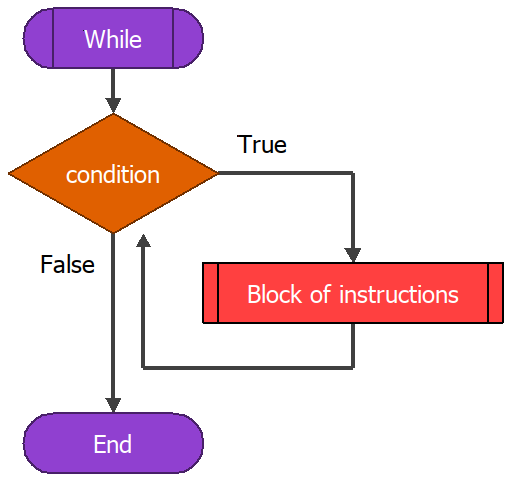
\includegraphics[scale=.24]{img/While_Chart.png}
\caption{while flowchart}
    \end{figure}
\end{frame}
\begin{frame}[fragile]{Loops}
    \tit{While loop with else}
    \texttt{while} loop can have an optional \text{else}. The \text{else} body is executed if the condition is \texttt{False} 
\begin{lstlisting}[numbers=left,showstringspaces=false,language=python]
counter = 0
while counter < 3:
    print("Inside while body")
    counter = counter + 1
else:
    print("Inside else body")
\end{lstlisting}        
\end{frame}
\begin{frame}[fragile]{Loops}
    \tit{\texttt{for} loops}
    \begin{itemize}
        \item The \texttt{for} loop allows to execute a block of instructions multiple times. In fact, this loop is used to iterate over iterable objects.
        \item An {\bf iterable objects} is a sequence of items capable of returning its members one by one, for example \texttt{list} and \texttt{strings} are iterable objects.
    \end{itemize}
    The \texttt{for} loop  syntax in python is:
\begin{lstlisting}[showstringspaces=false,language=python]
for loop_var in iterable_object:
    for_block #body
\end{lstlisting}   
The variable \texttt{loop\_var} take the values of the items of the iterable object. Loop continues until the variable reach the last item in the sequence.


The body of the loop must be indented.
% TODO: range() function
\end{frame}
\begin{frame}[fragile]{Loops}
    \exercise{Draw the flowchart of for loop}
% \begin{figure}
%         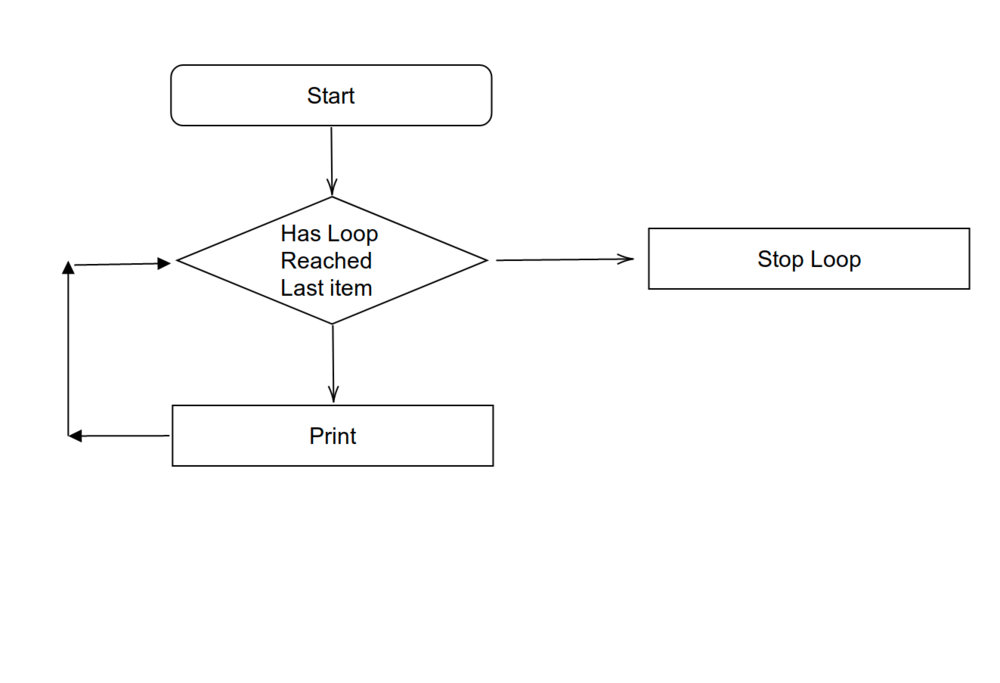
\includegraphics[scale=.24]{img/For_Chart.png}
% \caption{for flowchart}
%     \end{figure}
\tit{Example: Python \texttt{for} Loop}
\begin{lstlisting}[numbers=left,showstringspaces=false,language=python]
word="NHSM"
for letter in word:
    print(letter)
\end{lstlisting}        
\end{frame}
\begin{frame}[fragile]{Loops}
    \tit{\texttt{range()} function}
    In python, we can use the {range()} function to generate a sequence of numbers.
    \pause
    The usage of range function is as follows:
        $$\texttt{range([start], stop,[step\_size])}$$
\begin{align*}
    \texttt{start}: &\text{(Optional). An integer number specifying at which position to start.}\\ 
                    &\text{Default is 0.}\\
    \texttt{stop}:&\text{An integer number specifying at which position to stop}\\
                  & \text{(not included).}\\
    \texttt{step}:&\text{(Optional). An integer number specifying the incrementation.}\\
                  &\text{Default is 0.}
\end{align*}
\pause
    Try this
    \begin{lstlisting}[numbers=left,showstringspaces=false,language=python]
print(range(10))
print(list(range(10)))
print(list(range(2, 8)))
print(list(range(2, 20, 3)))
    \end{lstlisting}        
\end{frame}
\begin{frame}[fragile]{Loops}
    \tit{Examples}
    \begin{lstlisting}[numbers=left,showstringspaces=false,language=python]
        #example1
        for i in range(9):
            print(i)
        else:
            print("No items left.")
        #example2 (else)
        digits=[6,2,9]
        for digit in digits:
            print(digit)
        else:
            print("No items left.")
        #example3
        # Program to iterate through a list using indexing
        names = ['Omar', 'Mohamed', 'Ali']
        # iterate over the list using index
        for i in range(len(names)):
            print("His name is", names[i])
    \end{lstlisting}
\end{frame}
\begin{frame}[fragile]{Loops}
    \tit{Loops}
    \exercise{Write a program which print the following messages\\
    "Hi Student 1"\\
    "Hi Student 2"
    

    \hspace{1cm} \vdots\\
    "Hi Student 90"\\
    "Hi Student 100"}
   \pause

    Will you print all the messages using 100 \texttt{print} function?!! So What we can do ?
\pause    
    \begin{block}{}
        In programming, loops are the statements that allow executing the same block of instructions multiple times.


        Python has essentially two types of loops: \texttt{while loops} and \texttt{for loops}.
    \end{block}
\end{frame}
% \begin{frame}[fragile]{Loops}
%     \tit{}
%     \begin{lstlisting}[numbers=left,showstringspaces=false,language=python]
%     \end{lstlisting}        
% \end{frame}
% \begin{frame}[fragile]{Loops}
%     \tit{}
%     \begin{lstlisting}[numbers=left,showstringspaces=false,language=python]
%     \end{lstlisting}        
% \end{frame}
% \begin{frame}[fragile]{Loops}
%     \tit{}
%     \begin{lstlisting}[numbers=left,showstringspaces=false,language=python]
%     \end{lstlisting}        
% \end{frame}
% \begin{frame}[fragile]{Loops}
%     \tit{}
%     \begin{lstlisting}[numbers=left,showstringspaces=false,language=python]
%     \end{lstlisting}        
% \end{frame}
% \begin{frame}[fragile]{Loops}
%     \tit{}
%     \begin{lstlisting}[numbers=left,showstringspaces=false,language=python]
%     \end{lstlisting}        
% \end{frame}
% \begin{frame}[fragile]{Loops}
%     \tit{}
%     \begin{lstlisting}[numbers=left,showstringspaces=false,language=python]
%     \end{lstlisting}        
% \end{frame}%Conditions \& Loops
% TODO: pass,  break,  continue
%TODO: while Loop 
%TODO: for Loop 
%TODO: break and continue 
%TODO: Pass 
%TODO:Common errors in loops 

% \begin{frame}[fragile]{Loops}
%     \tit{While loops}
%  \begin{itemize}[<+->]
%     \item A \texttt{while} loop allows a block of instructions to execute as long as (or while) a condition is \texttt{True}.
%     \item When the condition is \texttt{False}, the loop's body is ignored, and the execution continues at the first statement after the body of the \texttt{while} loop.
%     \item The body of the while loop is determined through indentation.
%     \item If the condition always evaluates to \texttt{True}, the body will be executed infinitely, that's what we call {\bf infinite loop problem}.
%     \item We must update the condition's variables to avoid the infinite loop.
%     \item Generally, we use while loops when we don't know the number of executions of the loop's body.
% \end{itemize}
% \end{frame}
% \begin{frame}[fragile]{Loops}
% \tit{\texttt{while} syntax and flowchart}
%     \texttt{while}'s loop syntax is:



% \begin{lstlisting}[showstringspaces=false,language=python, caption={while syntax}]
% while (condition):
%     block_instructions #body
% \end{lstlisting}            
% \begin{figure}
%         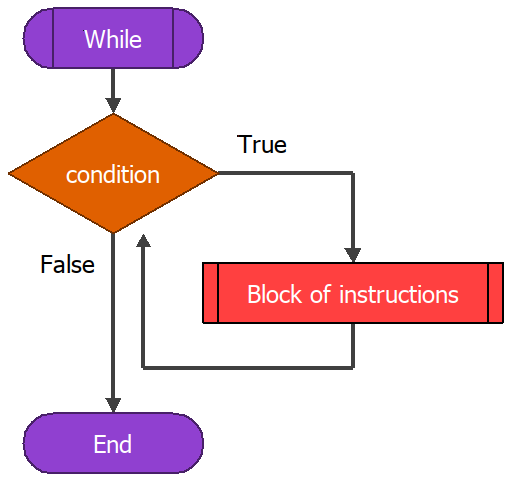
\includegraphics[scale=.24]{img/While_Chart.png}
% \caption{while flowchart}
%     \end{figure}
% \end{frame}
% \begin{frame}[fragile]{Loops}
%     \tit{While loop with else}
%     \texttt{while} loop can have an optional \text{else}. The \text{else} body is executed if the condition is \texttt{False} 
% \begin{lstlisting}[numbers=left,showstringspaces=false,language=python]
% counter = 0
% while counter < 3:
%     print("Inside while body")
%     counter = counter + 1
% else:
%     print("Inside else body")
% \end{lstlisting}        
% \end{frame}
% \begin{frame}[fragile]{Loops}
%     \tit{\texttt{for} loops}
%     \begin{itemize}
%         \item The \texttt{for} loop allows to execute a block of instructions multiple times. In fact, this loop is used to iterate over iterable objects.
%         \item An {\bf iterable objects} is a sequence of items capable of returning its members one by one, for example \texttt{list} and \texttt{strings} are iterable objects.
%     \end{itemize}
%     The \texttt{for} loop  syntax in python is:
% \begin{lstlisting}[showstringspaces=false,language=python]
% for loop_var in iterable_object:
%     for_block #body
% \end{lstlisting}   
% The variable \texttt{loop\_var} take the values of the items of the iterable object. Loop continues until the variable reach the last item in the sequence.


% The body of the loop must be indented.
% % TODO: range() function
% \end{frame}
% \begin{frame}[fragile]{Loops}
%     \exercise{Draw the flowchart of for loop}
% % \begin{figure}
% %         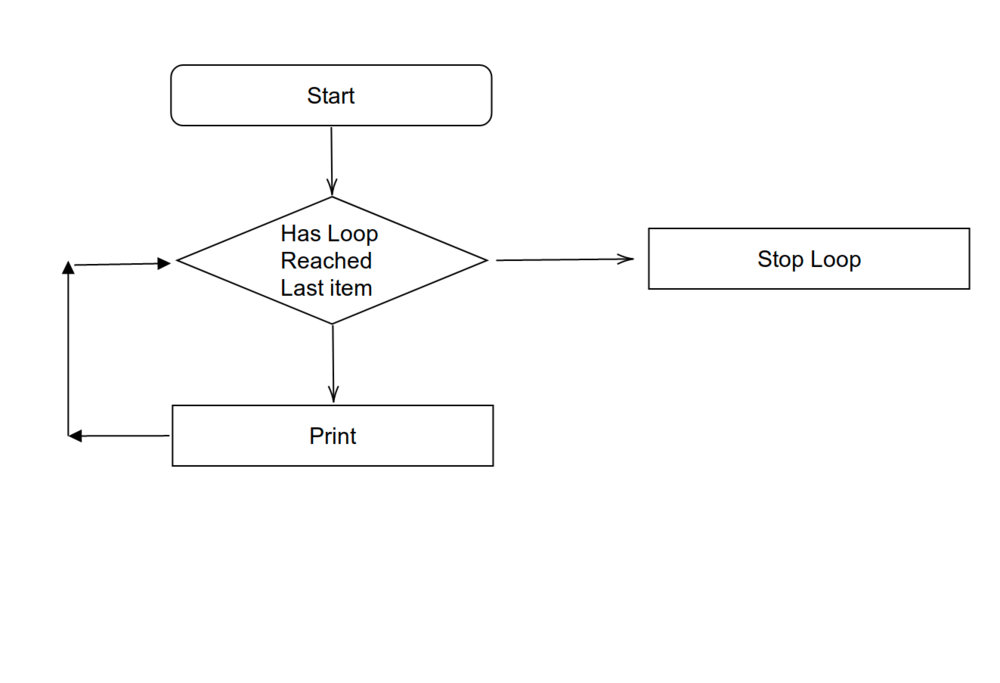
\includegraphics[scale=.24]{img/For_Chart.png}
% % \caption{for flowchart}
% %     \end{figure}
% \tit{Example: Python \texttt{for} Loop}
% \begin{lstlisting}[numbers=left,showstringspaces=false,language=python]
% word="NHSM"
% for letter in word:
%     print(letter)
% \end{lstlisting}        
% \end{frame}
\begin{frame}[fragile]{Loops}
    \tit{\texttt{range()} function}
    In python, we can use the {range()} function to generate a sequence of numbers.
    \pause
    The usage of range function is as follows:
        $$\texttt{range([start], stop,[step\_size])}$$
\begin{align*}
    \texttt{start}: &\text{(Optional). An integer number specifying at which position to start.}\\ 
                    &\text{Default is 0.}\\
    \texttt{stop}:&\text{An integer number specifying at which position to stop}\\
                  & \text{(not included).}\\
    \texttt{step}:&\text{(Optional). An integer number specifying the incrementation.}\\
                  &\text{Default is 0.}
\end{align*}
\pause
    Try this
    \begin{lstlisting}[numbers=left,showstringspaces=false,language=python]
print(range(10))
print(list(range(10)))
print(list(range(2, 8)))
print(list(range(2, 20, 3)))
    \end{lstlisting}        
\end{frame}
\begin{frame}[fragile]{Loops}
    \tit{Examples}

    \begin{lstlisting}[numbers=left,showstringspaces=false,language=python]
        #example1
        for i in range(9):
            print(i)
        else:
            print("No items left.")
        #example2 (else)
        digits=[6,2,9]
        for digit in digits:
            print(digit)
        else:
            print("No items left.")
        #example3
        # Program to iterate through a list using indexing
        names = ['Omar', 'Mohamed', 'Ali']
        # iterate over the list using index
        for i in range(len(names)):
            print("His name is", names[i])
    \end{lstlisting}
\end{frame}
\begin{frame}[fragile]{Loops}
    \tit{\texttt{break} and \texttt{continue} }
    \begin{itemize}[<+->]
        \item The \texttt{break} statement terminates the loop containing it. The program execute the statement immediately after the body of the loop.
        \item The \texttt{continue} statement is used to skip the rest of the code inside a loop for the current iteration only. Loop does not terminate but continues on with the next iteration.
    \end{itemize}
\onslide<1->\begin{lstlisting}[numbers=left,showstringspaces=false,language=python]
name="NHSM"
for letter in name:
    if (letter=='S'):
        break
    print(letter)
\end{lstlisting}
\onslide<2>
\begin{lstlisting}[numbers=left,showstringspaces=false,language=python]
    name="NHSM"
    for letter in name:
        if (letter=='S'):
            continue
        print(letter)
    \end{lstlisting}
\end{frame}
% \begin{frame}[fragile]{Loops}
%     \tit{}
%     \begin{lstlisting}[numbers=left,showstringspaces=false,language=python]
%     \end{lstlisting}        
% \end{frame}
% \begin{frame}[fragile]{Loops}
%     \tit{}
%     \begin{lstlisting}[numbers=left,showstringspaces=false,language=python]
%     \end{lstlisting}        
% \end{frame}
% \begin{frame}[fragile]{Loops}
%     \tit{}
%     \begin{lstlisting}[numbers=left,showstringspaces=false,language=python]
%     \end{lstlisting}        
% \end{frame}
% \begin{frame}[fragile]{Loops}
%     \tit{}
%     \begin{lstlisting}[numbers=left,showstringspaces=false,language=python]
%     \end{lstlisting}        
% \end{frame}
% \begin{frame}[fragile]{Loops}
%     \tit{}
%     \begin{lstlisting}[numbers=left,showstringspaces=false,language=python]
%     \end{lstlisting}        
% \end{frame} %
% \include{Lect_6} %
% \include{Lect_7} %Dictionaries
% \include{Lect_8}
% \include{Lect_9}
% \include{refs}%References
\end{document}